%!TEX root = ../dokumentation.tex

\chapter{Projektziel}
\todo{Projekt Vision}

\section{Projektanforderungen}
Zur Definition der Projektanforderungen wurden mehrere Usecase-Diagramme erstellt.

Zunächst soll der Benutzer auf einer Übersichtsseite ankommen.
Der Usecase dieser Übersichtsseite in in der Abbildung~\ref{fig:usecaseOverview} dargestellt.
\begin{figure}
    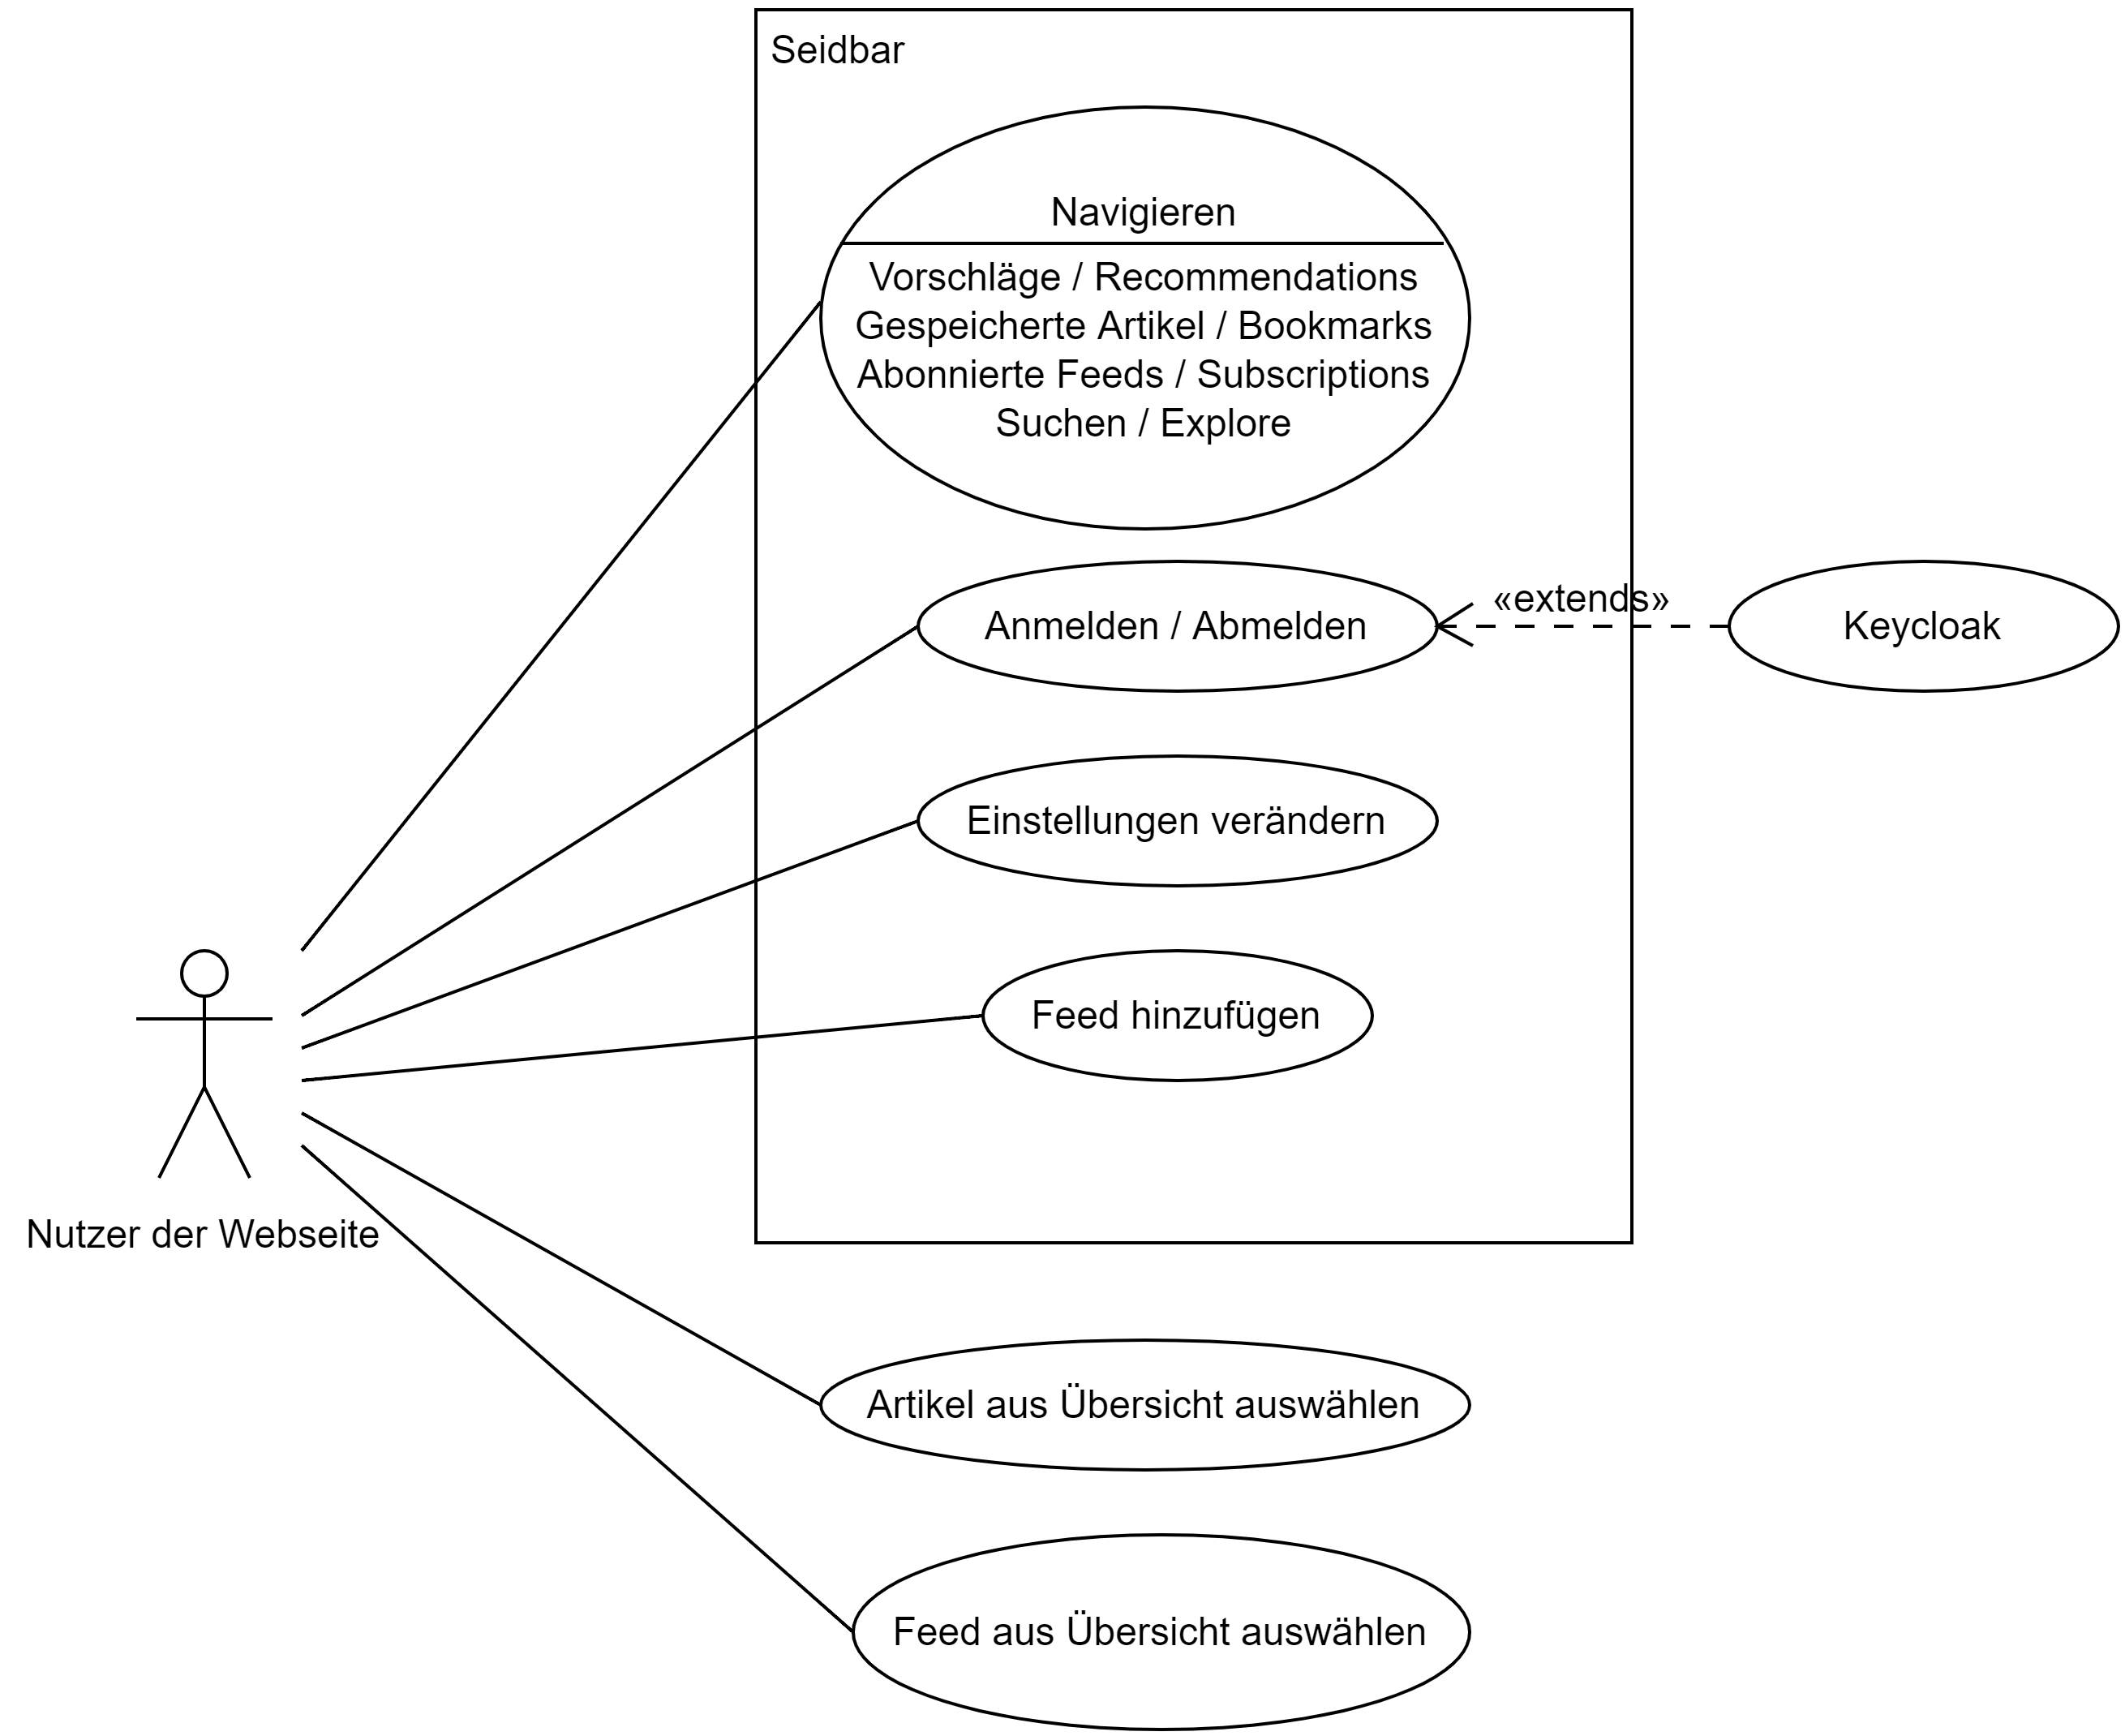
\includegraphics[width=\linewidth]{umlUsecaseOverview.png}
    \caption{Usecase Diagramm der Übersichtsseite}
    \label{fig:usecaseOverview}
\end{figure}
Auf dieser Übersichtsseite werden dem Nutzer verschiedene Feeds und Artikel angezeigt. Mit einem Klick auf einen Feed oder einen Artikel wird
der Nutzer auf eine weitere Seite weitergeleitet mit mehr Möglichkeiten. Außerdem hat der Nutzer auf der Seite über eine Sidebar die Möglichkeit
auf der Seite zu navigieren. Außerdem ist es in der Sidebar möglich seine Usereinstellungen zu ändern, sich an- und abmelden als auch neue Feeds
hinzuzufügen. 

Der Usecase der Einstellungsseite wurde in Abbildung~\ref{fig:usecaseSettings}
Auf dieser Seite ist ebenfalls die Sidebar, somit sind die Interaktionen in der Sidebar die selben, wie
bei der Übersichtsseite. Als weitere Funktionalität kann auf der kann man seinen Account
ändern. Dies soll über den externen Service Keycloak geschehen. Darüber hinaus
kann man Einstellungen zu Benachrichtigungen treffen. Außerdem kann das Design der
Webseite angepasst werden.
\begin{figure}
    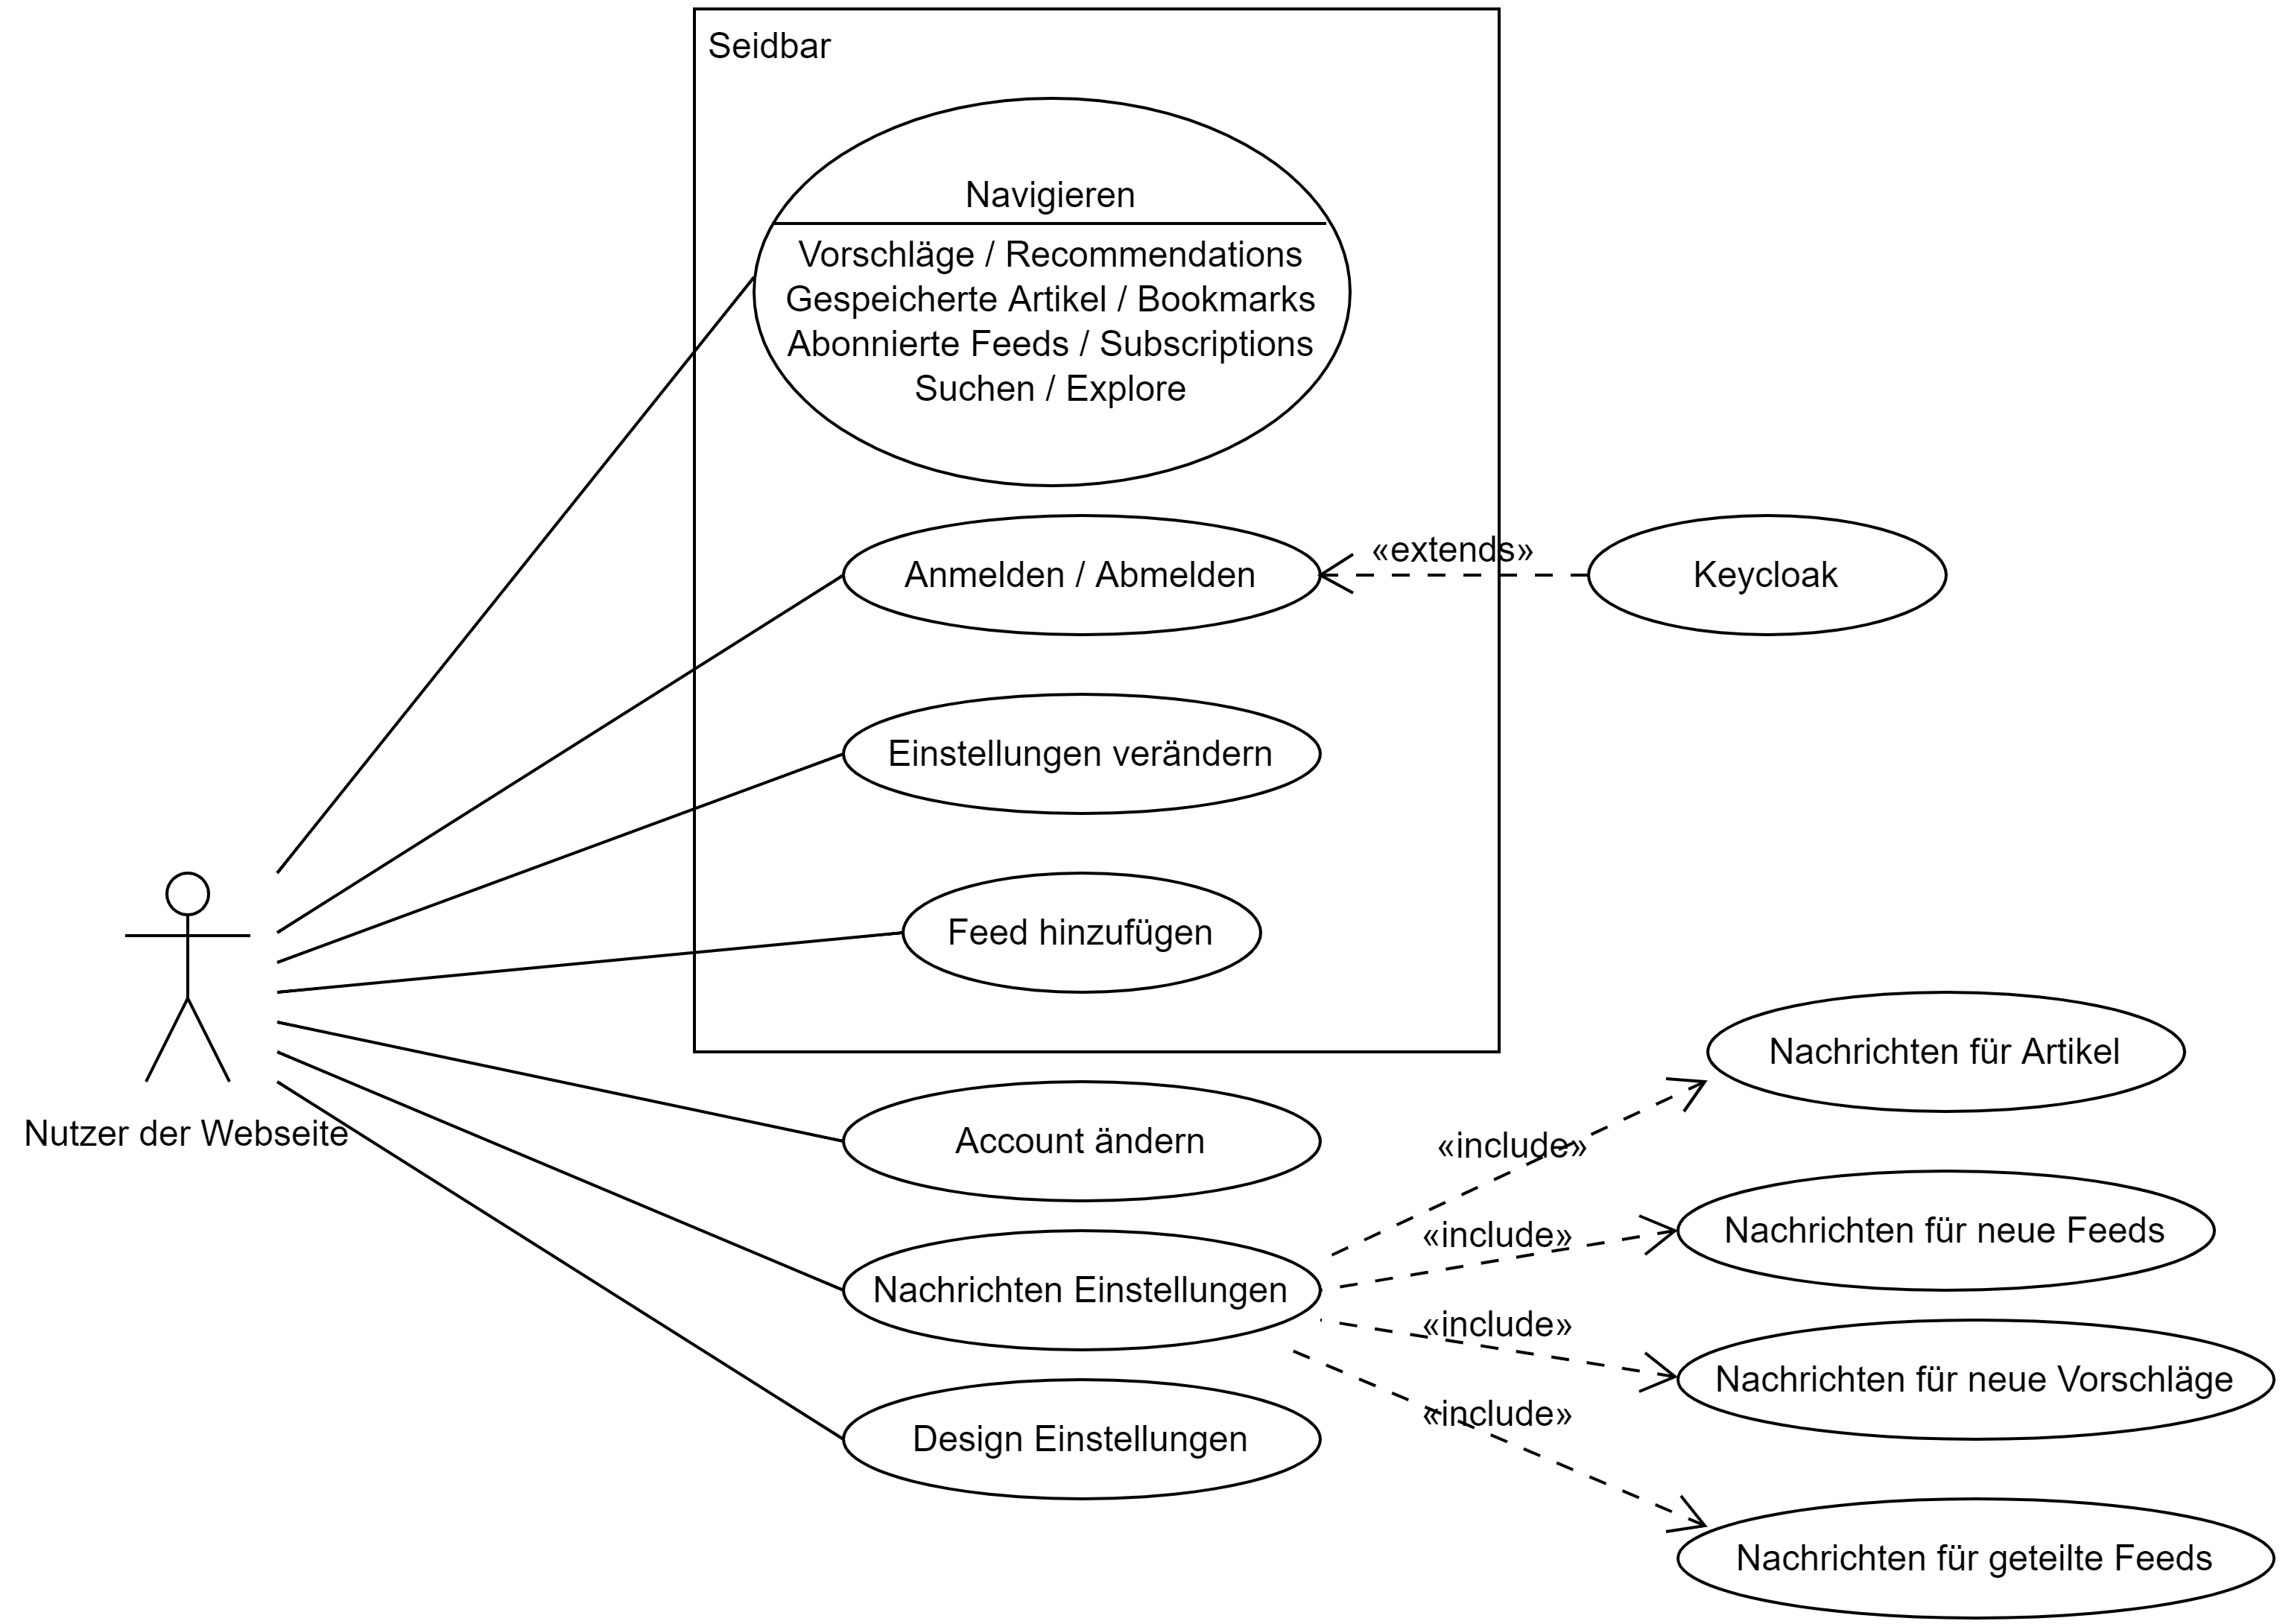
\includegraphics[width=\linewidth]{umlUsecaseSettings.png}
    \caption{Usecase Diagramm der Einstellungsseite}
    \label{fig:usecaseSettings}
\end{figure}


Es wurde ebenfalls ein Usecase Diagramm der Artikelseite angelegt. Auf diese Seite
wird der Nutzer weitergeleitet, falls er aus der Übersichtsseite einen Artikel anschaut.
Der Usecase der Artikelseite ist in der Abbilung~\ref{fig:usecaseView} dargestellt.
\begin{figure}
    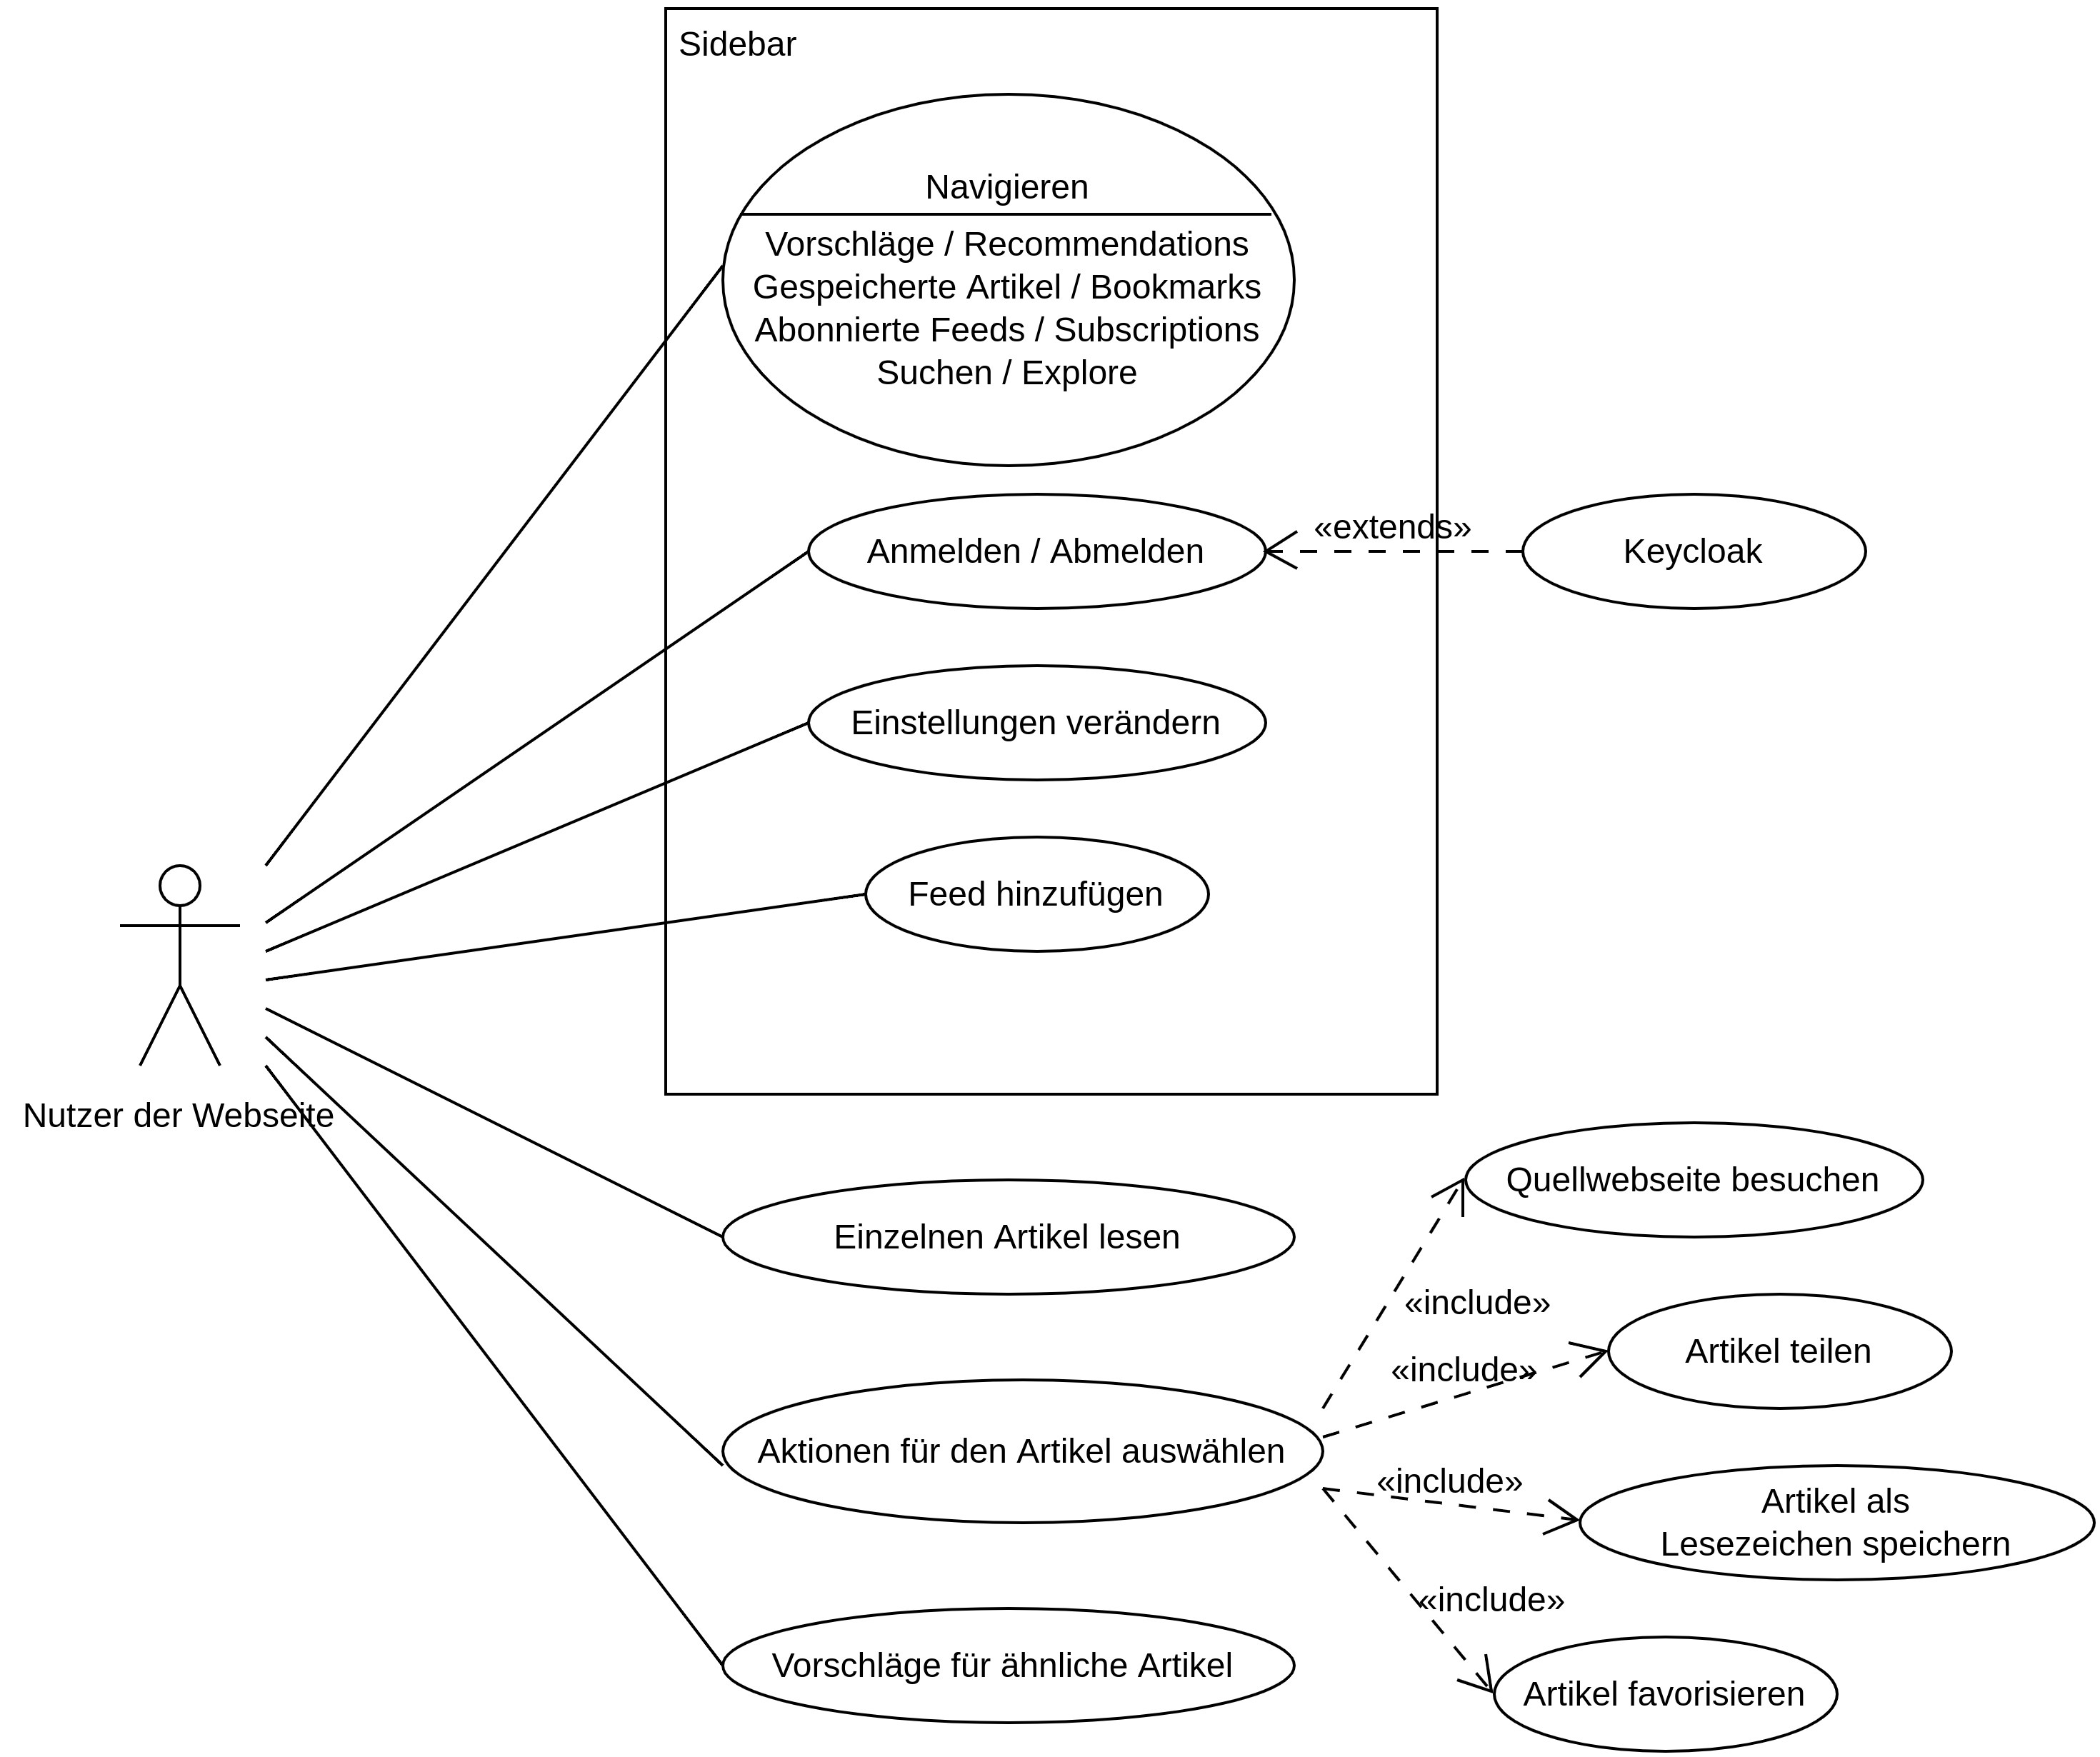
\includegraphics[width=\linewidth]{umlUsecaseView.png}
    \caption{Usecase Diagramm der Artikelseite}
    \label{fig:usecaseView}
\end{figure}
Zudem kann ein Benutzer verschiedene Aktionen auswählen, dazu zählen Quellwebseite des Artikels besuchen, Artikel teilen, Artikel als 
Lesezeichen speichern und Artikel favorisieren. Unterhalb der Aktionen werden Artikel angezeigt, die aufgrund bisheriger Präferenzen und 
favorisierten Artikeln passen könnten.

\subsection{Unverzichtbare Ziele}

\subsection{Erreichbare Ziele}

\subsection{Mögliche weiteren Ziele}

\section{Anfängliche Software Architektur}
\todo{Services etc beschreiben}
\todo{Software Auswahl beschreiben (express, angular)}
